\documentclass[conference]{IEEEtran}
\IEEEoverridecommandlockouts
% The preceding line is only needed to identify funding in the first footnote. If that is unneeded, please comment it out.
\usepackage{cite}
\usepackage{amsmath,amssymb,amsfonts}
\usepackage{algorithmic}
\usepackage{graphicx}
\usepackage{textcomp}
\usepackage{xcolor}
\usepackage{array}
\usepackage{hyperref}
\usepackage{multirow}
\usepackage{multicol}
\usepackage[lined,boxed,commentsnumbered]{algorithm2e}
\def\BibTeX{{\rm B\kern-.05em{\sc i\kern-.025em b}\kern-.08em
		T\kern-.1667em\lower.7ex\hbox{E}\kern-.125emX}}
\begin{document}
	
	\title{Optimization of Matrix Multiplication on CPU}
	
	\author{\IEEEauthorblockN{1\textsuperscript{st} Jiacheng Luo}
		\IEEEauthorblockA{\textit{dept. Computer Science and Engineering} \\
			\textit{Southern University of Science and Technology}\\
			Shenzhen, China \\
			12112910@mail.sustech.edu.cn}
	}
	
	\maketitle
	
	\begin{abstract}
		Matrix multiplication is a crucial operation that finds its applications in many subfields of computer science, such as machine learning, image processing, computer graphics, scientific computing, and cryptography. However, the naive algorithm for matrix multiplication fails to utilize hierarchical memories (multi-layer caches) efficiently, affecting its overall efficacy. To address this problem, we propose several techniques, such as loop reordering, matrix blocking with instruction sets and parallelizing, to improve the efficiency of matrix multiplication in classical modern computers with hierarchical memories. Furthermore, we indicate that the utilization rate of the computer cache is a critical constraint that affects the speed of matrix multiplication. Additionally, we present an implementation of fast CPU matrix multiplication. Our method is approximately 2000 times faster than the naive one as demonstrated through extensive experiments conducted on randomly generated single-precision floating-point matrices.
	\end{abstract}
	
	\begin{IEEEkeywords}
		matrix multiplication, hierarchical memories, efficiency, CPU implementation
	\end{IEEEkeywords}
	
	\section{Introduction}
	Matrix multiplication is a fundamental mathematical operation that is widely used in many areas of science, engineering, and computer science. Its importance arises from its wide range of applications, particularly in linear transformations, solving linear equations, data analytics, and signal processing. 
	
	The naive matrix multiplication algorithm has a time complexity of $\Theta(n^3)$ and does not fully utilize the hierarchical cache architecture of modern computers, leading to low efficiency when computing matrix multiplication on the CPU.
	
	This paper discovered that appropriately adjusting the loop order in the naive algorithm can enhance the cache utilization efficiency and subsequently improve the efficiency by approximately 10-fold. Additionally, further improvements to computational efficiency, up to approximately 2000 times, can be achieved through matrix blocking, instruction set optimization (such as SIMD or NEON), and the use of parallelization techniques (such as OpenMP). Moreover, this paper discusses a matrix multiplication algorithm with a time complexity of $\Theta(n^{\log_2 7})$, identifies its limitations, and discourages its use as a practical engineering tool for matrix multiplication.
	
	We used several randomly generated single-precision floating-point matrices for experiments.
	
	The main contributions of this work are summarized as follows:
	
	\begin{itemize}
		\item The efficiency of the naive algorithm can be improved by approximately 10-fold by simply adjusting the loop order, and this paper will explain why.
		\item This paper proposes a matrix multiplication algorithm with a time complexity of $\Theta(n^{\log_2 7})$, but this study discourages its use as a practical engineering tool for matrix multiplication.
		\item To improve the efficiency of matrix multiplication, this paper recommends implementing matrix blocking, optimizing instruction sets and employing parallelization techniques.
		\item  To illustrate such improvements, a CPU implementation was conducted using C. We conduct extensive experiments on randomly generated single-precision floating-point matrices and show that the proposed method speed up by 2000 times compared to the naive method.
	\end{itemize}

	\section{Related Work}
	\subsection{Divide-and-conquer Algorithm}
	By employing the divide-and-conquer algorithm, we can effectively accomplish the multiplication of two $2^n \times 2 ^ n$ matrices, where $n \geq 1$. Here, submatrices $A_{i,j}$, $B_{i,j}$, and $C_{i,j}$, where $1 \leq i,j \leq 2$, have a dimension of $2^{n - 1} \times 2^{n - 1}$, and subsequently, $C = A \times B$. \cite{b1}
	\begin{equation}\nonumber
		\resizebox{0.5\textwidth}{!}{$C=\left(\begin{array}{ll}C_{11} & C_{12} \\ C_{21} & C_{22}\end{array}\right), A=\left(\begin{array}{ll}A_{11} & A_{12} \\ A_{21} & A_{22}\end{array}\right), B=\left(\begin{array}{ll}B_{11} & B_{12} \\ B_{21} & B_{22}\end{array}\right)$}
	\end{equation}

	
	\begin{equation}
		\resizebox{0.44\textwidth}{!}{$\left(\begin{array}{ll}C_{11} & C_{12} \\ C_{21} & C_{22}\end{array}\right)=\left(\begin{array}{ll}A_{11} B_{11}+A_{12} B_{21} & A_{11} B_{12}+A_{12} B_{22} \\ A_{21} B_{11}+A_{22} B_{21} & A_{21} B_{12}+A_{22} B_{22}\end{array}\right)$}
	\end{equation}

	
	The time complexity of the algorithm is $\Theta(n^3)$ if we multiply two $n \times n $ matrices.
	\subsection{Cache Behavior}
	The efficiency of the matrix multiplication algorithm relies on the storage format of the matrix, which could be in row first, column first, or mixed. The efficiency of the algorithm could vary depending on the chosen storage format. Also, the order can have a considerable impact on practical performance due to the memory access patterns and cache use of the algorithm.\cite{b2} The optimal variant of the iterative algorithm for two $n \times n$ matrices $A$ and $B$ in row-major layout is a tiled version, where the matrix is implicitly divided into square tiles of size $\sqrt{M}$ by $\sqrt{M}$. \cite{b3} In the idealized cache model, this algorithm incurs only $ \Theta(\frac{n^3}{b\sqrt{M}})$ cache misses; the divisor $b\sqrt{M}$ amounts to several orders of magnitude on modern machines, so that the actual calculations dominate the running time, rather than the cache misses.
	\section{Preliminary}
	\subsection{Matrix Multiplication}
	Matrix multiplication is an operation that takes two matrices and produces a third matrix. Given two matrices $A$ and $B$, where $A$ has $m$ rows and $n$ columns, and B has $n$ rows and $p$ columns, their product $C$ is an $m$ by $p$ matrix. The $(i,j)$-th entry of $C$ is given by the sum of the products of all elements in the $i$-th row of $A$ and the $j$-th column of $B$:
	
	\begin{equation}
		C_{i,j} = \sum_{k=1}^{n} A_{i,k} B_{k,j}
	\end{equation}
	
	
	Here, $\sum$ denotes summation, $k$ ranges over all common indices for row $i$ in $A$ and column $j$ in $B$. The indices $i$ and $j$ represent the row and column of the product matrix $C$, respectively.
	
	\subsection{Execution Time}
	Matrix multiplication execution time refers to the amount of time it takes for a computer to perform the matrix multiplication operation. The time is typically measured in seconds or milliseconds.
	
	The execution time of matrix multiplication depends on multiple factors, including the size of the matrices being multiplied, the hardware (such as processor speed and memory bandwidth) on which the multiplication is being performed, and the implementation of the multiplication algorithm.
	
	One way to calculate the execution time of matrix multiplication is to measure the time taken to execute each step of the algorithm, including memory allocation, data initialization, computation, and memory deallocation. This can be done using different tools such as profilers or timers.
	
	The formula for calculating the execution time of matrix multiplication can be expressed as:
	
	\begin{equation}
		\resizebox{0.44\textwidth}{!}{
			$Time_{Execution} = Time_{Multiplication} + Time_{MemoryOperations}$
		}
	\end{equation}
	
	
	The time for multiplication refers to the time taken to perform the actual matrix multiplication, while the time for memory operations includes the time taken for memory allocation, data initialization, and memory deallocation.
	
	\subsection{FLOP} 
	
	FLOP (floating-point operations per second) is a measure of a computer's performance in terms of floating-point arithmetic. It is defined as the number of floating-point operations (additions, subtractions, multiplications, and divisions) that a computer can perform in one second.
	
	It is often expressed in terms of gigaflops (billions of FLOPS) or teraflops (trillions of FLOPS), depending on the system's performance. The formula for calculating FLOP (floating-point operations per second) in terms of mathematical notation is as follows:
	
	\begin{equation}
		FLOP = \frac{N \times F}{T}
	\end{equation}
	
	
	Where $N$ represents the number of floating-point operations, $F$ represents the number of CPU clock cycles required for each floating-point operation, and $T$ represents the time taken to complete the computation (typically measured in seconds).
	
	The value of $F$ can be calculated using the following formula:
	
	\begin{equation}
		F = \frac{CPU \ Clock \ Cycles}{Floating \ Point \ Operation}
	\end{equation}
	
	
	Where CPU Clock Cycles represents the number of CPU clock cycles required to execute each floating-point operation, and Floating Point Operation represents the number of CPU instructions or micro-operations required to execute each floating-point operation.
	
	Therefore, the formula for calculating FLOP can be written as:
	
	\begin{equation}
		FLOP = \frac{N \times CPU \ Clock \ Cycles}{T \times Floating \ Point \ Operation}
	\end{equation}
	
	
	This formula represents the number of floating-point operations that can be performed per second on a computer.
	
	\section{Our Method}
	In this section, we first propose modifying the loop order of the naive algorithm as a means of reducing cache misses while providing theoretical derivation to support the proposal. Subsequently, we suggest additional cache reduction through the implementation of blocked algorithms to accelerate matrix multiplication. We next introduce the Strassen's algorithm, which exhibits low theoretical time complexity, and analyze its time complexity while explaining why it is not widely used in industry. Finally, we optimize matrix multiplication calculations using a combination of matrix blocking, parallel computing, and instruction set optimization techniques.
	
	\subsection{Reordering Loops}
	We define the size of matrices involved in matrix multiplication as $n \times n$ for convenience. To compute the product $C_{i,j}$ with the naive implementation (in sequence: $i, j, k$), we must multiply the $i$-th row of matrix $A$ with the $j$-th column of matrix $B$. Due to the storage arrangement in the Matrix library, accessing memory is continuous when we move rightward within the corresponding row of $A$, but not when we move downward within the column of $B$. By computing $C_{i,j}$, we repeatedly access column $B$ discontinuously for $n$ times, while we access row $A$ discontinuously only once (when returning to the beginning). Therefore, the total number of jumps equals to $n^3 + n^2$. As the matrix is stored as a one-dimensional array, we do not have to jump when we complete the calculation of $C_{i,n}$, and thus the total number of jumps needed equals to $n^3 + n^2 - n$.
	
	Changing the order of the loop to $i,k,j$ for the computation of $C_{i,j}$ multiplies the $i$-th row of matrix $A$ with the $j$-th column of matrix $B$. As a result of storing the matrices by row in the Matrix library, memory access is continuous both when we move rightward within the corresponding row of $A$ and when we move downward within the corresponding column of $B$. Therefore, the total number of jumps for computation of $C_{i,j}$ equals to $n^2$.
	
	Similarly, for different loop orders, we calculate the total number of jumps as shown in the Table ~\ref{tab:loopjumps}:
	
	\begin{table}[htbp]
		\caption{Number of Jumps for Different Loop Orders}
		\centering\
		\setlength\extrarowheight{2pt}
		\label{tab:loopjumps}
		\begin{tabular}{|c|c|}
			\hline
			Loop Order & Number of Jumps \\ \hline
			$i,k,j$ & $n^2$ \\ \hline
			$k,i,j$ & $2n^2$ \\ \hline
			$j,i,k$ & $n^3 + n^2 + n$ \\ \hline
			$i,j,k$ & $n^3 + n^2 - n$ \\ \hline
			$k,j,i$ & $2n^3$ \\ \hline
			$j,k,i$ & $2n^3 + n^2$ \\ \hline
		\end{tabular}
	\end{table}
	
	The large size of matrices presents a significant constraint on computational speed due to the inherent problem of memory access continuity in naive algorithms. Yet, simply swapping the loop order can enhance memory continuity and improve computational efficiency.By conducting theoretical analysis and selecting the optimal loop order, the program's efficiency in accessing memory continuity increases by a factor of approximately $n$ when compared to the naive algorithm.
	
	Consequently, optimizing memory continuity to ensure continuous program access maximizes computational efficiency and extracts the full computational capacity of the central processing unit (CPU).
	\subsection{Matrix Blocking}
	Matrices $A_{m \times k}$ and $B_{k \times n}$ can be multiplied to result in matrix $C_{m \times n}$. By using a batching method, we multiply a batch of $m_R$ rows of matrix $A$ with a batch of $n_R$ columns of matrix $B$ to obtain a partial matrix of size $m_R \times n_R$. This partial matrix is a part of the final result matrix $C$.
	
	\begin{figure}[htbp]
		\centerline{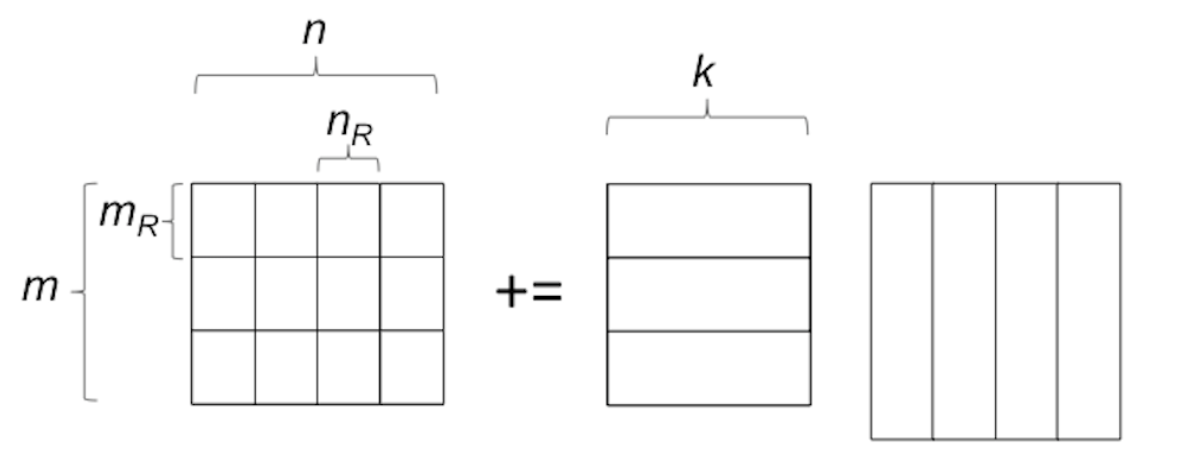
\includegraphics[width=0.45\textwidth]{fig1.png}}
		\caption{Matrix Blocking Flowchart Diagram}
		\label{matrixBlockingOverall}
	\end{figure}
	
	\subsubsection{matmul\underline{\ }blockMatrix\underline{\ }2x2(matrix1, matrix2)}
	We designed an algorithm which implements the aforementioned conceptual approach by specifying $m_R = 2$ and $n_R = 2$. For the implementation of the above algorithm, we have conducted memory access optimizations such as loop unrolling and storing $2 \times 2$ computation results in registers. It should be noted that due to the slightly larger constant in the block matrix division process when compared to naive loops, the experimental effects may not be as pronounced without the aforementioned memory access optimizations. 
	\subsubsection{matmul\underline{\ }blockMatrix(matrix1, matrix2)}
	Additionally, we devised a more general matrix block multiplication algorithm which calculates a matrix multiplication by partitioning the matrices. Nonetheless, since the inner layer of this algorithm comprises a variable-sized matrix of dimensions $m_R \times n_R$, both loop unrolling and in-register intermediate result storage are infeasible.
	
	 Consequently, for the $m_R = n_R = 2$ case, this algorithm's computational efficiency may be slightly inferior to the above-defined algorithm due to the constant factor. Nevertheless, the significance of this algorithm lies in the flexibility to manually select dimensions of the block matrices and investigate the correlation between block matrix sizes and algorithmic efficiency.
	 
	 \subsection{Strassen's Algorithm}
	 In terms of optimizing the divide-and-conquer approach, we presented an algorithm with lower computational complexity, known as the Strassen's algorithm \cite{b5}.
	 
	 Assuming matrices $A, B$ are both square matrices of size $N \times N (N = 2 ^ n)$, if we want to calculate the product of matrices $C = A \times B$, we can perform block division on the matrices. Specifically, we can represent $A$ and $B$ as $\begin{bmatrix}
	 	A_{11} & A_{12}\\
	 	A_{21} & A_{22}
	 \end{bmatrix}$ and $\begin{bmatrix}
	 	B_{11} & B_{12}\\
	 	B_{21} & B_{22}
	 \end{bmatrix}$ respectively, and represent $C$ as $\begin{bmatrix}
	 	C_{11} & C_{12}\\
	 	C_{21} & C_{22}
	 \end{bmatrix}$.
 
 Then we can use the following formulas:
	 $$C_{11} = A_{11} \cdot B_{11} + A_{12} \cdot B_{21}, C_{12} = A_{11} \cdot B_{12} + A_{12} \cdot B_{21}$$
	 $$C_{21} = A_{21} \cdot B_{11} + A_{22} \cdot B_{21}, C_{22} = A_{21} \cdot B_{12} + A_{22} \cdot B_{22}$$
	 By using the above formulas recursively, we can compute the product of two matrices of size $n \times n$ with 2 matrices of size $\frac{n}{2} \times \frac{n}{2}$ through 8 multiplications and 4 additions, making the time complexity $T(n) = 8 T(\frac{n}{2}) + \Theta(n^2)$, which is $\Theta(n^3)$ in general. However, using Strassen's algorithm can reduce the number of multiplications to 7.
	 
	 To do that, we define $S_1, ..., S_{10}$ as:
	 ​ $$S_1 = B_{12} - B_{22}, S_2 = A_{11} + A_{12}$$ $$S_3 = A_{21} + A_{22}, S_4 = B_{21} - B_{11}$$ $$S_5 = A_{11} + A_{22}, S_6 = B_{11} + B_{22}$$ $$S_7 = A_{12} - A_{22}, S_8 = B_{21} + B_{22}$$ $$S_9 = A_{11} - A_{21}, S_{10} = B_{11} + B_{12}$$
	 And $P_1, ..., P_{7}$ as:
	 ​ $$P_1 = A_{11}S_1, P_2 = S_2B_{22}, P_3 = S_3B_{11}, P_4 = A_{22}S_4$$ $$P_5 = S_5S_6, P_6 = S_7S_8, P_7 = S_9S_{10}$$
	 Then we can get:
	 ​ $$C_{11} = P_5 + P_4 - P_2 + P_6, C_{12} = P_1 + P_2$$ $$C_{21} = P_3 + P_4, C_{22} = P_5 + P_1 - P_3 - P_7$$
	 
	 Using the above algorithm, computing the product of two matrices of size $n \times n$ requires 7 multiplications and 18 additions of two matrices of size $\frac{n}{2} \times \frac{n}{2}$, making the time complexity $T(n) = 7 T(\frac{n}{2}) + \Theta(n^2)$, which is $\Theta(n^{\log_2 7})$ in general. By combining Strassen's algorithm with the optimization of changing the loop order (i.e., when the number of rows of matrix after block division is less than a certain value, the product is directly calculated using brute force), we can further optimize the performance of matrix multiplication, for example we can set the value of this threshold to be 128 when the matrix size is greater than 128.
	 
	 Although Strassen's algorithm has some inherent drawbacks, it is not completely unsuitable for use as a matrix multiplication library. However, care needs to be taken into consideration due to the following reasons:
	 
	\begin{itemize}
\item Strassen's algorithm is only faster than the naive algorithm on larger matrices. Therefore, it should only be used on matrices that are large enough.

\item The constant factor in Strassen's algorithm is larger than that of the naive algorithm, so for small-scale data, the naive algorithm may be faster.

\item Strassen's algorithm requires more computation and memory, and the trade-off between speed and memory usage should be carefully considered.

\item Padding may be needed to convert non-square matrices to square matrices, which may increase the computational cost of the algorithm.

\item If in-place calculation is desired, a proper memory management strategy should be adopted to avoid excessive memory usage.
	 \end{itemize}
	 
	 \subsection{Matrix Blocking with Instruction Set Optimization and Parallelization Techniques}
	 
	 In the previous discussion, we attempted to optimize the multiplication process by fitting the matrices into registers to reuse their data extensively. However, as the value of $K$ becomes larger, when accessing the $m_R \times K$ and $K \times n_R$ submatrices, there is also a high probability of experiencing cache misses. From experimental data, it can be observed that this optimization has an insignificant effect on matrices larger than $256$.
	 
	 In this section, we aim to improve the efficiency of the program by copying the discontiguous data to contiguous memory and fetching from contiguous memory during computation, thereby reducing the probability of cache misses.
	 
	 Suppose we aim to implement the multiplication of two matrices $A_{m \times k}$ and $B_{k \times n}$, to obtain the matrix $C_{m\times n}$, as shown in the Fig.~\ref{matrixBlockingStep0}.
	 
	 \begin{figure}[htbp]
	 	\centerline{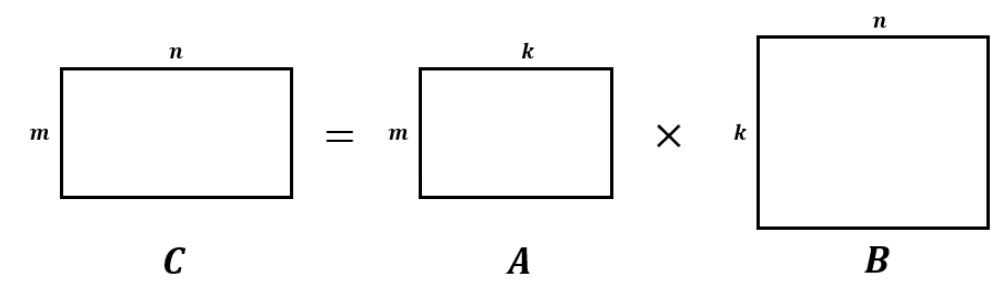
\includegraphics[width=0.5\textwidth]{fig2.png}}
	 	\caption{Matrix Blocking Step (0)}
	 	\label{matrixBlockingStep0}
	 \end{figure}
 
 	Firstly, we partition the $n$ dimension into blocks of size $n_C$, and each block is processed individually as shown in the Fig.~\ref{matrixBlockingStep1}.
 	
	\begin{figure}[htbp]
		\centerline{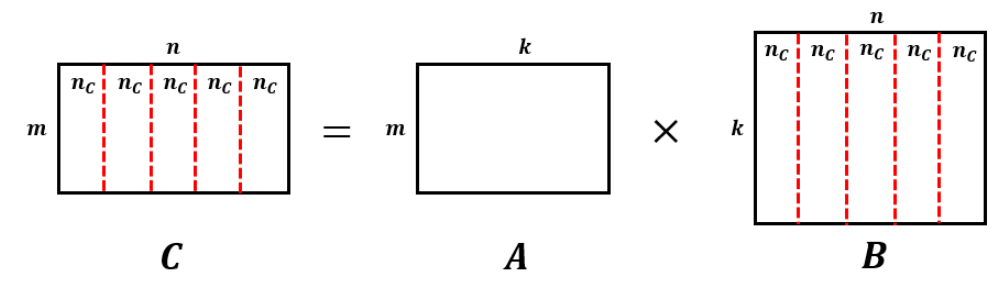
\includegraphics[width=0.5\textwidth]{fig3.png}}
		\centerline{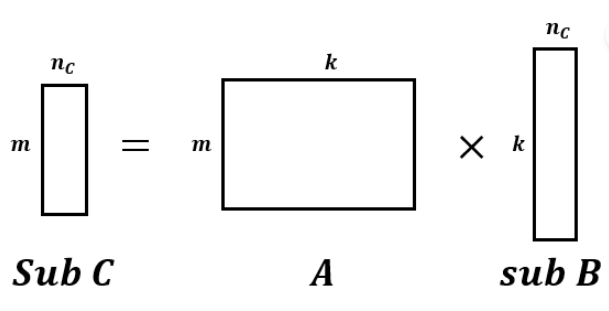
\includegraphics[width=0.3\textwidth]{fig3-2.png}}
		\caption{Matrix Blocking Step (1)}
		\label{matrixBlockingStep1}
	\end{figure} 

 	Then, we partition the $k$ dimension into blocks of size $k_C$, and each block is processed individually as shown in the Fig.~\ref{matrixBlockingStep2}.
	
	\begin{figure}[htbp]
		\centerline{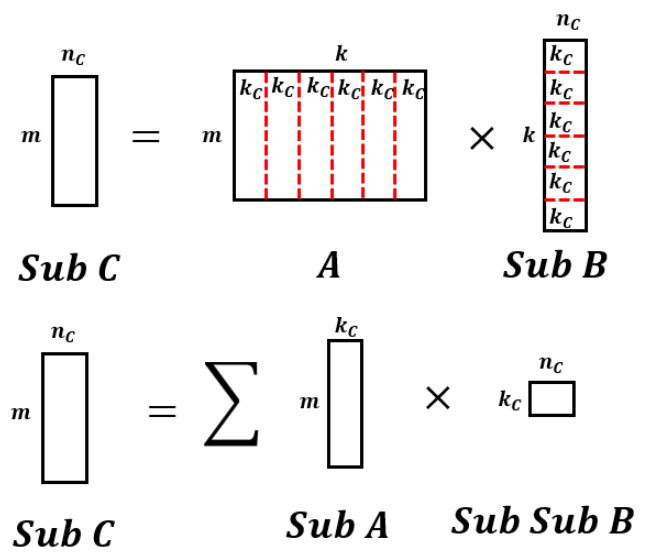
\includegraphics[width=0.4\textwidth]{fig4.png}}
		\caption{Matrix Blocking Step (2)}
		\label{matrixBlockingStep2}
	\end{figure}

 	Then, we partition the $m$ dimension into blocks of size $m_C$, and each block is processed individually as shown in the Fig.~\ref{matrixBlockingStep3}.
 	
	\begin{figure}[htbp]
	\centerline{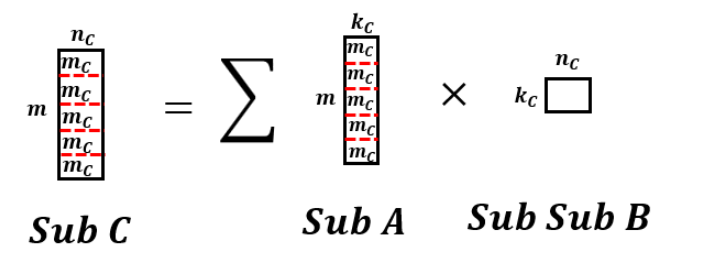
\includegraphics[width=0.5\textwidth]{fig5.png}}
	\centerline{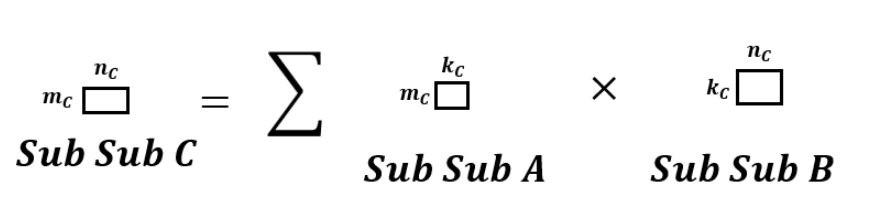
\includegraphics[width=0.4\textwidth]{fig5-2.png}}
	\caption{Matrix Blocking Step (3)}
	\label{matrixBlockingStep3}
	\end{figure}

	To compute a $m_C \times k_C$ matrix and a $k_C \times n_C$ matrix, we employ the matrix partitioning method mentioned earlier (i.e. defining $n_R = m_R = 2$, but in general, we can customize the values of $n_R$ and $m_R$) to optimize the computation process.
	
	The aforementioned technique involves copying discontinuous data into contiguous memory and accessing it for computation from the contiguous memory. To achieve this, we can pack ``sub sub A" and ``sub sub B", as shown in the Fig.~\ref{matrixBlockingStep4}.
	
	\begin{figure}[htbp]
		\centerline{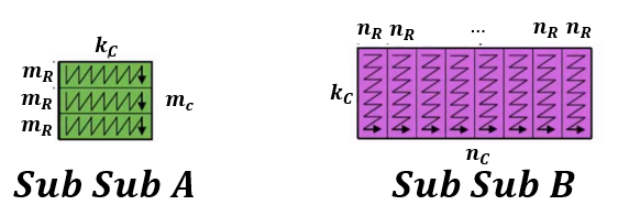
\includegraphics[width=0.4\textwidth]{fig6-1.png}}
		\centerline{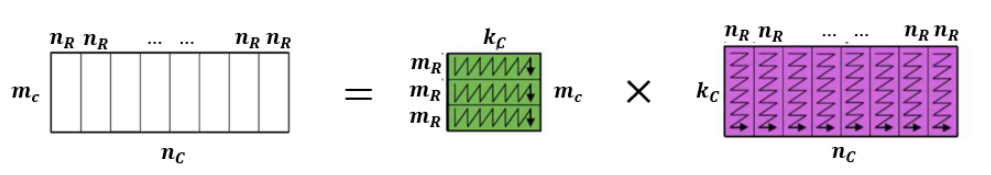
\includegraphics[width=0.5\textwidth]{fig6-2.png}}
		\centerline{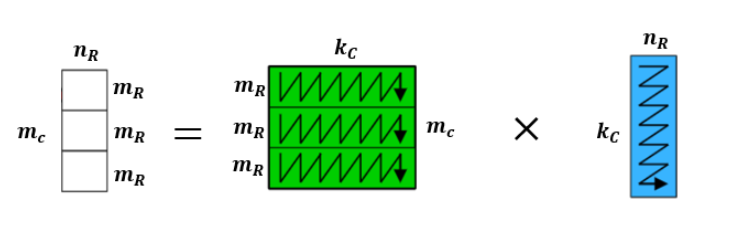
\includegraphics[width=0.4\textwidth]{fig6-3.png}}
		\centerline{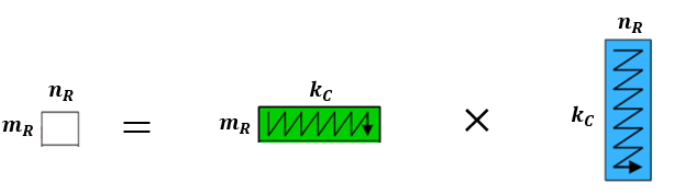
\includegraphics[width=0.4\textwidth]{fig6-4.png}}
		\caption{Matrix Blocking Step (4)}
		\label{matrixBlockingStep4}
	\end{figure}

	To calculate $n_R \times m_R$, the result can be initially stored in a register, and once the $k_C$ floating-point operations have completed, the result can then be moved from the register to the original memory location.
	
	We further optimized the above algorithm by utilizing parallelization and instruction sets.
	
	\subsubsection{Parallelization}
	The optimizations mentioned above were only executed using a single core of the CPU or a single process, without utilizing all the cores available in the computer. Based on algorithms such as loop permutation, matrix partitioning, and matrix packing, it is evident that we calculate each part of the matrix separately, and these parts are indeed independent of each other, which makes them highly suitable for parallel computation. By employing instructions that enable parallel execution of these parts, we can significantly increase the efficiency of the calculations. Fortunately, many compilers support OpenMP, which can be easily used by adding the relevant compilation parameters without requiring additional installation.
	\subsubsection{Instruction Set Optimization}
	When calculating the products of smaller matrices, $m_R \times k_C$ and $k_C \times n_R$, they can be viewed as the dot products of $m_R$ row vectors and $n_R$ column vectors, respectively, where each vector has a length of $k_C$. Utilizing SIMD/NEON instruction sets can optimize this process, determined by whether the computer employs an ARM or x86 architecture.
	
	
	\section{Experiments}
	
	In the experimental section, we randomly generated a single precision floating-point matrix of size $n \times n$ for experimentation. Firstly, we conducted experiments by changing the loop order of the naive algorithm. We used multiple datasets of different sizes and compared the execution time of the two loop sequences that resulted in the least and the most cache misses, respectively. Then, we used multiple datasets of varying sizes to test the execution time of Strassen's algorithm and matrix multiplication with blocking and parallel instructions optimized. We also compared the relative accuracy of each method and explained the reasons for our observations. Finally, we implemented the matrix multiplication library designed for CPU using C on the x86 and ARM platforms and compared the running efficiency of the two platforms. The source code is open source at \url{https://github.com/Maystern/SUSTech_CS201_Matrix_Multiplication}.
	
	\subsection{Platform}
	To compare the efficiency of matrix multiplication on different platforms, we conducted experiments on three platforms, as shown in table~\ref{tab:system_config1}, ~\ref{tab:system_config2} and ~\ref{tab:system_config3}. Please note that unless otherwise specified, the experiments will be tested on the x86 server ``x86 Server Platform: CVIP Server" without any compiler optimization flags.
	
	\begin{table}[htbp]
		 \centering
		 \begin{minipage}[t]{\linewidth}
		 	\centering
		 	\caption{x86 PC Platform: Lenovo Xiaoxin Pro 16}
		 	\label{tab:system_config1}
		 	\setlength\extrarowheight{2pt}
		 	\begin{tabular}{|c|c|}
		 		\hline
		 		Item & Information                                                                               \\ \hline
		 		Architecture & x86\_64                                                                            \\ \hline
		 		CPU              & $1$ $8$-core CPU, AMD Ryzen 7 5800H \\ 
		 		& with Radeon Graphics  @ $3.20$ GHz                                                                 \\ \hline
		 		Memory     & $16$ GB                                                                                     \\ \hline
		 		Cache            & $512$ KB (L1 Cache), $4$ MB (L2 Cache), \\
		 		& $16$ MB (L3 Cache)           \\ \hline
		 	\end{tabular}
		\end{minipage}
	 	\hspace{\linewidth}
	 	\begin{minipage}[t]{\linewidth}
	 		\centering
	 		\caption{x86 Server Platform: CVIP Server}
	 		\label{tab:system_config2}
	 		\setlength\extrarowheight{2pt}
	 		\begin{tabular}{|c|c|}
	 			\hline
	 			Item & Information \\ \hline
	 			Architecture & x86\_64 \\ \hline
	 			CPU & $4$ $14$-core CPU, Intel(R) \\ 
	 			& Xeon(R) Gold 6132 CPU @ 2.60GH \\ \hline
	 			Memory & 512 GB \\ \hline
	 			Cache & 896 KB (L1 Cache), 8.0 MB (L2 Cache), \\ 
	 			& 38.5 MB (L3 Cache) \\ \hline
	 		\end{tabular}
	 	\end{minipage}	
 		\hspace{\linewidth}
 		\begin{minipage}[t]{\linewidth}
 			\centering
 			\caption{ARM PC Platform: MacBook Air M1}
 			\label{tab:system_config3}
 			\setlength\extrarowheight{2pt}
 			\begin{tabular}{|c|c|}
 				\hline
 				Item & Information \\ \hline
 				Architecture & arm\_64 \\ \hline
 				CPU & 1 $8$-core CPU, model Apple M1 Pro \\ 
 				& @ 3.35 GHz \\ \hline
 				Memory & 16 GB \\ \hline
 				Cache & 192 KB (L1 Cache) $4.0$ MB (L2 Cache) \\ \hline
 			\end{tabular}
 		\end{minipage}	
	\end{table}

	
	\subsection{Change the Loop Order}
	
	Two different methods, $i,k,j$ and $j,k,i$, were utilized to perform the experiment. As anticipated by the theory, the former demonstrated significantly higher speed compared to the latter. The experiment results are presented in Table ~\ref{tab:matrix-mult-perf} and Figure.~\ref{fig::loop order}.
	
	\begin{table}[h]
		\centering
		\caption{Loop Order Optimization}
		\label{tab:matrix-mult-perf}
		\setlength\extrarowheight{2pt}
		\begin{tabular}{|c|c|c|c|}
			\hline
			Matrix Size & $j, k, i$ Time(ms) & $i, k, j$ Time(ms) & Ratio \\ \hline
			1          & $1.76\times 10^{-4}$       & $1.08\times 10^{-4}$         & 1.63              \\ 
			2          & $2.52\times 10^{-4}$       & $1.32\times 10^{-4}$         & 1.91              \\ 
			4          & $6.35\times 10^{-4}$       & $4.26\times 10^{-4}$         & 1.49              \\ 
			8          & $3.20\times 10^{-3}$       & $2.64\times 10^{-3}$         & 1.21              \\ 
			16         & $2.32\times 10^{-2}$       & $1.96\times 10^{-2}$         & 1.19              \\ 
			32         & $1.81\times 10^{-1}$       & $1.50\times 10^{-1}$         & 1.21              \\ 
			64         & 1.44                        & 1.18                         & 1.22              \\
			128        & 12.4                        & 9.65                         & 1.29              \\
			256        & $1.09\times 10^{2}$        & $7.64\times 10^{1}$          & 1.42              \\ 
			512        & $1.40\times 10^{3}$        & $6.15\times 10^{2}$          & 2.27              \\ 
			1024       & $1.55\times 10^{4}$        & $4.90\times 10^{3}$          & 3.17              \\ 
			2048       & $1.60\times 10^{5}$        & $3.91\times 10^{4}$          & 4.10              \\ 
			4096       & $2.29\times 10^{6}$        & $3.08\times 10^{5}$          & 7.43              \\ 
			8192       & $2.45\times 10^{7}$        & $2.47\times 10^{6}$          & 9.95              \\ 
			\hline
		\end{tabular}
	\end{table}
	
	\begin{figure}[htbp]
		\centerline{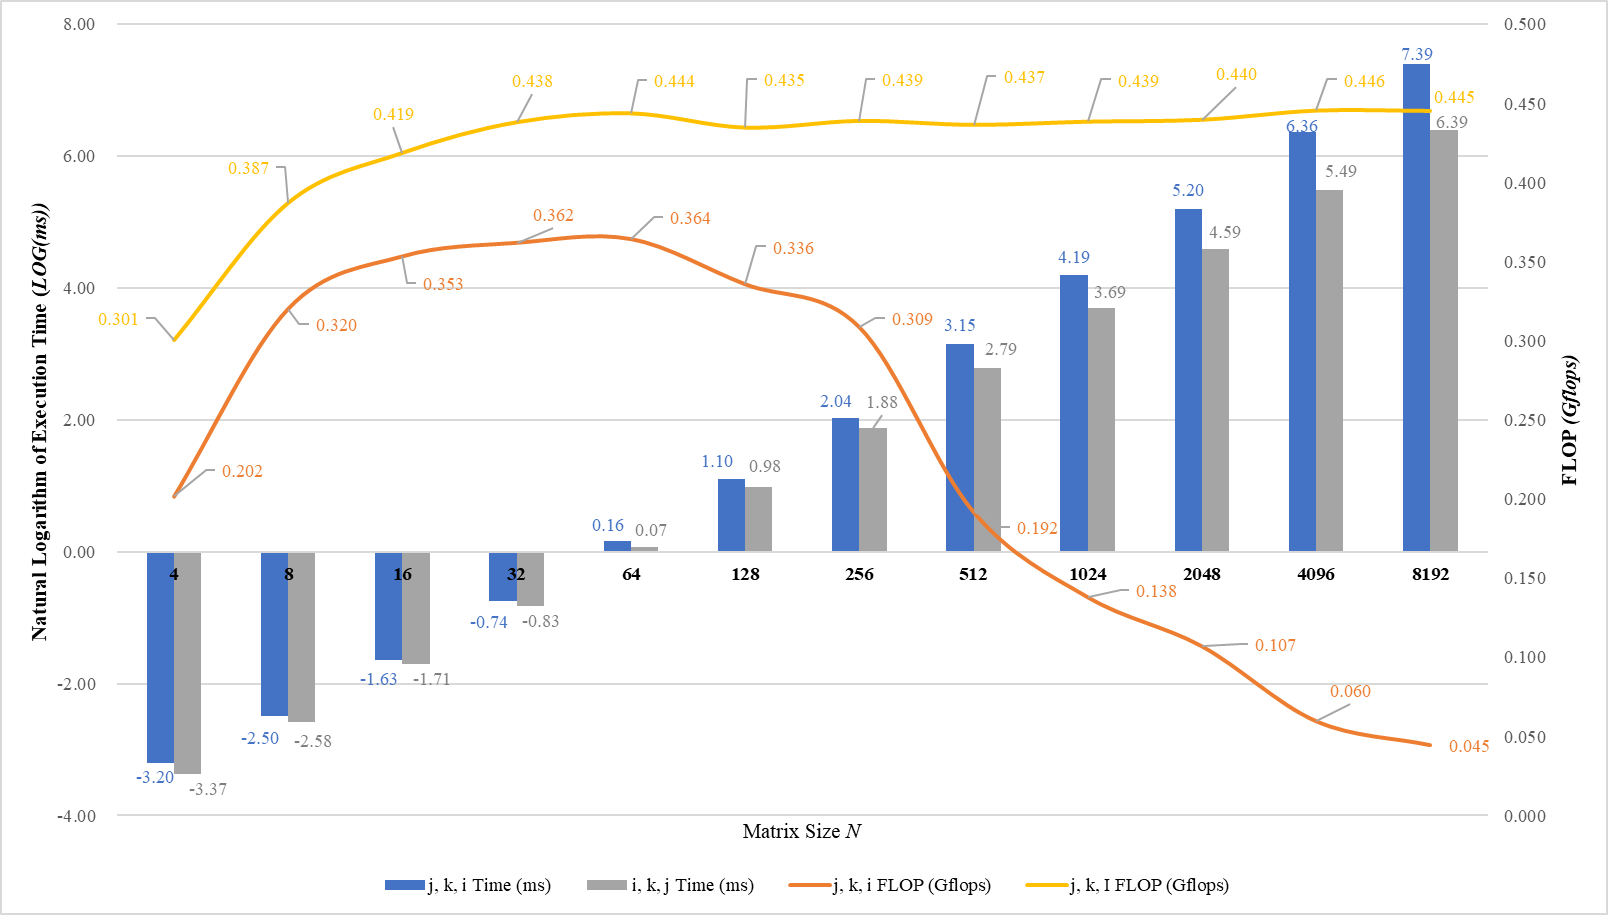
\includegraphics[width=0.5\textwidth]{fig7.png}}
		\caption{Loop Order Optimization}
		\label{fig::loop order}
	\end{figure}

	From the figure above, the following conclusions can be drawn:
	
	\subsubsection{With the increase in matrix size, the time consumption of both algorithms increases. However, the loop optimization algorithm performs better than the naive brute-force algorithm, taking lesser time} This is possibly due to the fact that both algorithms have a complexity of $\Theta(n^3)$, but the loop optimization algorithm is better at accessing memory continuity than the naive brute-force algorithm.
	
	\subsubsection{	With the increase in matrix size, changes in the floating-point frame rate of both algorithms differ:
		The floating-point frame rate of the naive brute-force algorithm first increases and then decreases, while that of the loop optimization algorithm first increases and then gradually stabilizes} This is likely due to the problem of memory continuity that significantly affects the calculation speed of the naive brute-force algorithm at larger matrix sizes, whereas the loop optimization algorithm mitigates this limitation. Theoretical analysis shows that the loop optimization algorithm is roughly $n$ times more efficient than the naive brute-force algorithm in terms of accessing memory continuity, and this effect is increasingly evident as the data size increases.
	
	\subsection{Strassen's Algorithm}
	We obtained the data presented in Table ~\ref{table:NaiveStrassenAlgorithm} for matrix multiplication using Strassen's algorithm for matrices of size less than or equal to $128$.
	
	\begin{table}[h]
		\centering
		\caption{Strassen's Algorithm (1)}
		\label{table:NaiveStrassenAlgorithm}
		\setlength\extrarowheight{2pt}
		\resizebox{0.5\textwidth}{!} {
		\begin{tabular}{|c|c|c|c|}
			\hline
			\textbf{Matrix Size} & \textbf{Naive Time(ms)} & \textbf{Strassen' s Algorithm Time(ms)} & \textbf{Ratio} \\ \hline
			1 & $1.76 \times 10^{-4}$ & $1.82 \times 10^{-4}$ & 0.967 \\
			2 & $2.52\times 10^{-4}$ & $4.00 \times 10^{-3}$ & 0.063 \\
			4 & $6.35 \times 10^{-4}$ & $3.41\times 10^{-2}$ & 0.018 \\
			8 & $3.20 \times 10^{-3}$ & $2.35 \times 10^{-1}$ & 0.014 \\
			16 & $2.32 \times 10^{-2}$ & 1.70 & 0.014 \\
			32 & $1.81 \times 10^{-1}$ & $1.17 \times 10^{1}$ & 0.015 \\
			64 & 1.44 & $8.29 \times 10^{1}$ & 0.017 \\
			128 & 12.4 & $5.83 \times 10^2$ & 0.021 \\ \hline
		\end{tabular}
	}
	\end{table}
	
	After implementing the Strassen's algorithm, we discovered that the efficiency was actually worse than the naive algorithm. We posit that this is due to the many intermediate matrix variables defined during the algorithm's execution, coupled with the fact that the optimization effect of the algorithm is not apparent when dealing with smaller datasets. Therefore, for larger matrix multiplications, we replaced the calculation of multiplying two matrices smaller than 128 in size within the Strassen algorithm's execution process with the $\Theta(n^3)$ algorithm that utilizes a changed loop order as we had previously done. Experimental results showed that this optimization significantly improved the Strassen algorithm's efficiency.
	
	The experiment results are presented in Table ~\ref{table:StrassenAlgorithm} and Figure.~\ref{fig::strassen}.
	
	\begin{table}[h]
		\centering
		\caption{Strassen's Algorithm (2)}
		\label{table:StrassenAlgorithm}
		\setlength\extrarowheight{2pt}
		\resizebox{0.5\textwidth}{!} {
		\begin{tabular}{|c|c|c|c|}
			\hline
			\textbf{Matrix Size} & \textbf{Naive Time(ms)} & \textbf{Strassen's Algorithm Time(ms)} & \textbf{Ratio} \\ \hline
			256 & $1.09 \times 10^2$ & $7.41\times 10^{1}$ & 1.47 \\ 
			512 & $1.40 \times 10^3$ & $5.48 \times 10^2$ & 2.54 \\ 
			1024 & $1.55 \times 10^{4}$ & $3.89 \times 10^3$ & 3.99 \\ 
			2048 & $1.60 \times 10^5$ & $2.78 \times 10^4$ & 5.77 \\ 
			4096 & $2.29 \times 10^6$ & $1.94 \times 10^5$ & 11.80 \\ 
			8192 & $2.45 \times 10^7$ & $1.37 \times 10^6$ & 17.96 \\ \hline
		\end{tabular}
	}
	\end{table}
	
	\begin{figure}[htbp]
		\centerline{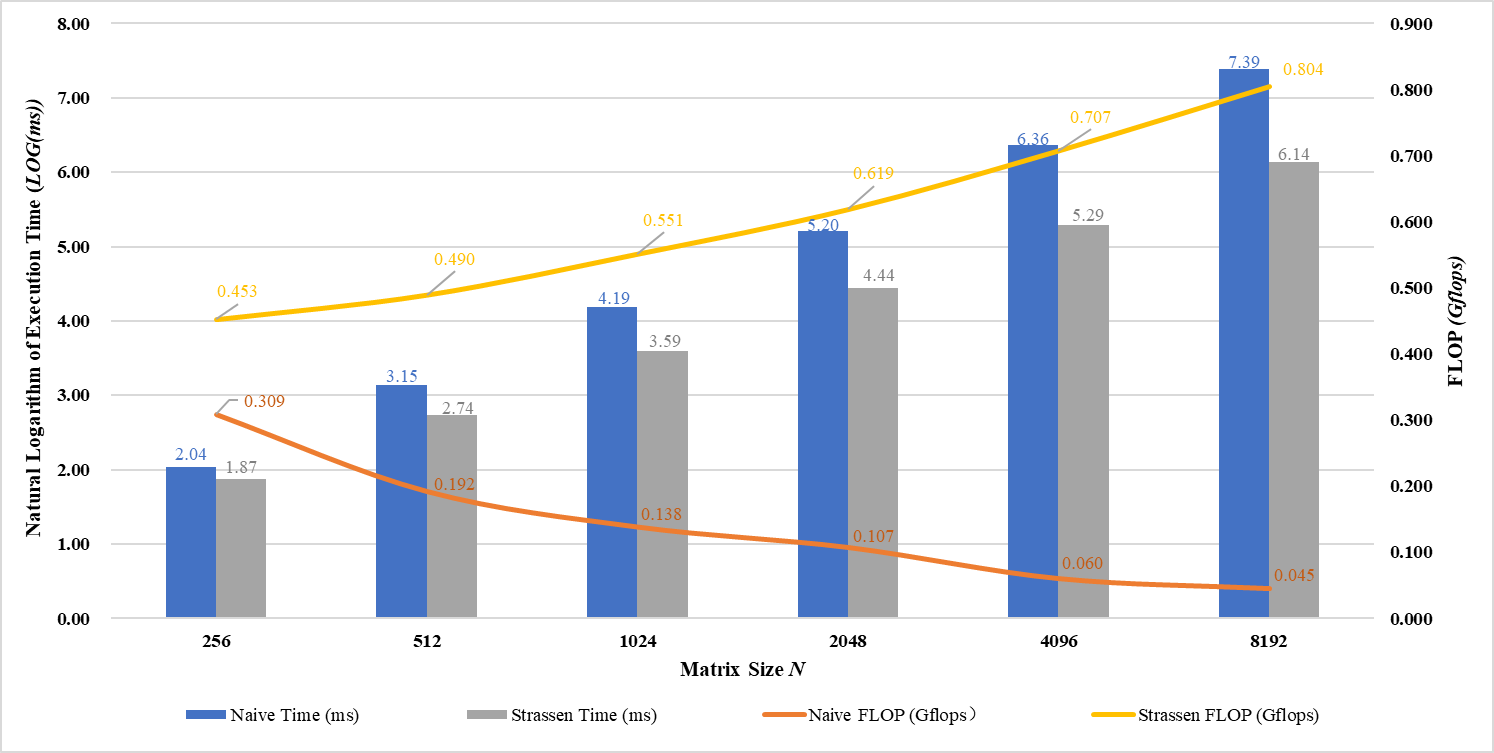
\includegraphics[width=0.5\textwidth]{fig8.png}}
		\caption{Strassen's Algorithm}
		\label{fig::strassen}
	\end{figure}

	Based on the experiments carried out above, the following conclusions can be drawn:
	
	Implementing the Strassen's algorithm can significantly reduce the time complexity of matrix multiplication from $\Theta(n^3)$ to $\Theta(n^{\log_2 7})$, resulting in a considerable improvement in efficiency for large-scale matrix computations. For relatively small matrix sizes, the Strassen's algorithm is slower due to its constant factor. Therefore, optimised algorithms with better performance should be used in such cases. The Strassen's algorithm has a stable increase in floating-point frame rate with the increase of data size, making it a viable option for medium to large matrices.
	
	\subsection{Matrix Blocking with Instruction Set Optimization and Parallelization Techniques}
	
	This optimisation represents the final version of the optimisation performed in this paper. It combines the ideas of loop reordering and matrix tiling by making memory contiguous and maximising cache hit rates. The optimisation overcomes the limitations of the Strassen algorithm, which often results in increased complexity instead of theoretical complexity reduction. This final version uses matrix packing optimisation, parallelisation (OpenMP), and instruction set optimisation (SIMD/NEON). We believe this optimisation presents an exceptional matrix multiplication solution. Subsequent testing confirms that this optimisation performs better, particularly for large matrix sizes, significantly improving the efficiency of matrix multiplication operations.
	
	The experiment results are presented in Table ~\ref{tab:matrixfinal} and Figure.~\ref{fig::matrixfinal}.
	
	\begin{table}[h]
		\centering
		\setlength\extrarowheight{2pt}
		\caption{Matrix Blocking with Instruction Set Optimization and Parallelization Techniques}
		\label{tab:matrixfinal}
		\begin{tabular}{|c|c|c|c|}
			\hline
			Matrix Size & Naive Time(ms)& Optimized Time(ms) & Rate \\ \hline
			1 & $1.76 \times 10^{-4}$ & $1.21 \times 10^{1}$ & 0.00 \\ 
			2 & $2.52\times 10^{-4}$ & $1.28 \times 10^{1}$ & 0.00 \\ 
			4 & $6.35 \times 10^{-4}$ & $1.21\times 10^{1}$ & 0.00 \\ 
			8 & $3.20 \times 10^{-3}$ & $1.26 \times 10^{1}$ & 0.00 \\ 
			16 & $2.32 \times 10^{-2}$ & $1.26 \times 10^{1}$ & 0.00 \\ 
			32 & $1.81 \times 10^{-1}$ & $1.29 \times 10^{1}$ & 0.01 \\ 
			64 & 1.44 & $1.24 \times 10^{1}$ & 0.12 \\ 
			128 & 12.4 & $1.23 \times 10^{1}$ & 1.01 \\ 
			256 & $1.09 \times 10^{2}$ & $1.30 \times 10^{1}$ & 8.39 \\ 
			512 & $1.40 \times 10^{3}$ & $2.39\times 10^{1}$ & 58.47 \\ 
			1024 & $1.55 \times 10^{4}$ & $5.39 \times 10^{2}$ & 288.00 \\ 
			2048 & $1.60 \times 10^{5}$ & $2.45 \times 10^{2}$ & 653.48 \\ 
			4096 & $2.29 \times 10^{6}$ & $1.59 \times 10^{3}$ & 1441.56 \\ 
			8192 & $2.45 \times 10^{7}$ & $1.10 \times 10^{4}$ & 2224.27 \\ \hline
		\end{tabular}
	\end{table}
	
	\begin{figure}[htbp]
		\centerline{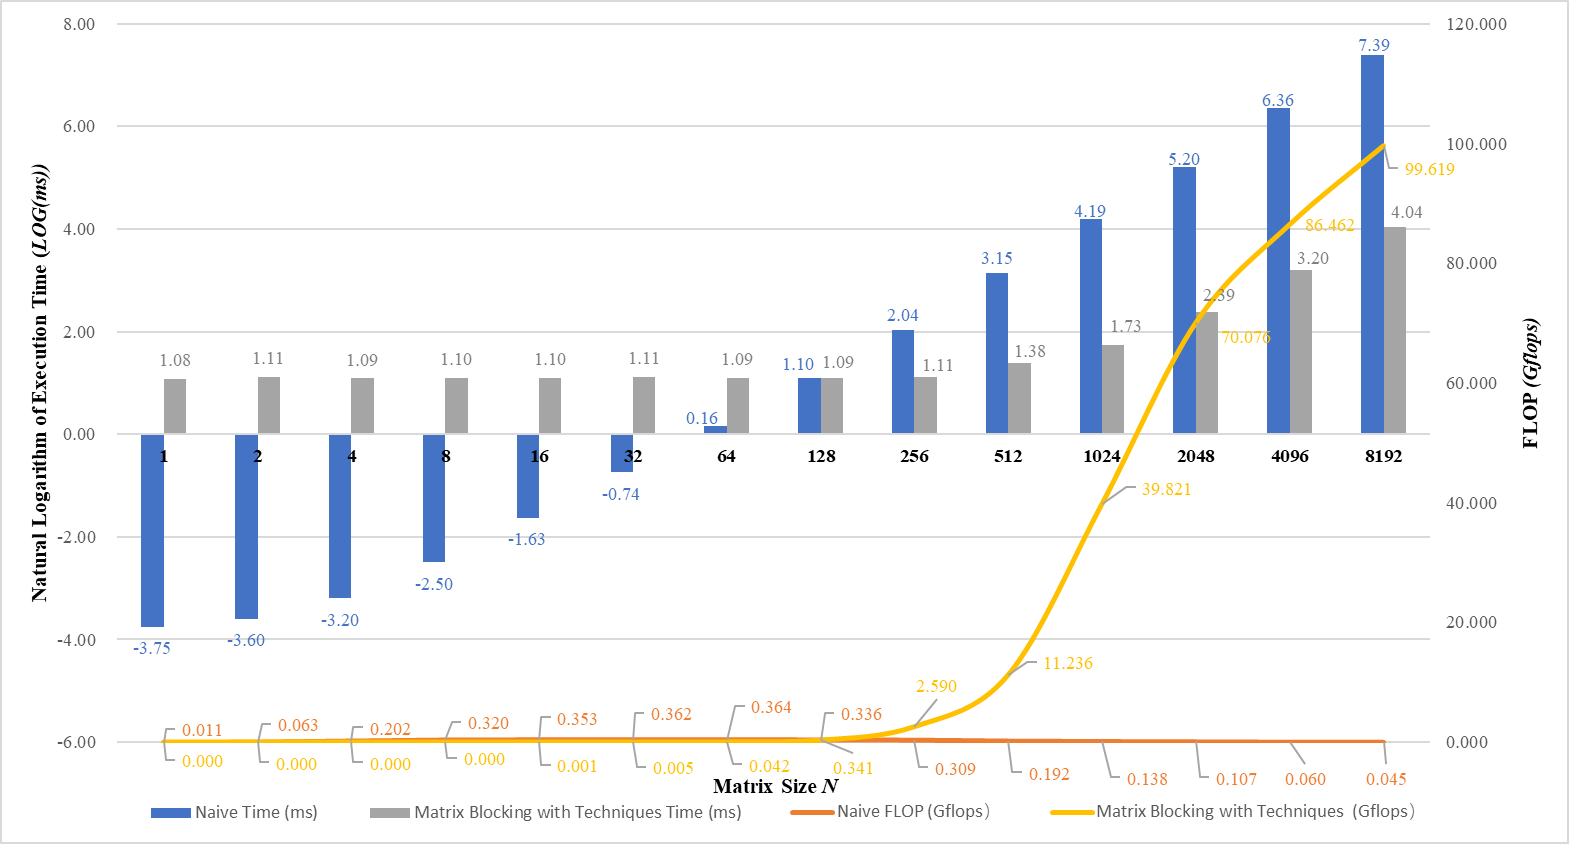
\includegraphics[width=0.5\textwidth]{fig9.png}}
		\caption{Matrix Blocking with Instruction Set Optimization and Parallelization Techniques}
		\label{fig::matrixfinal}
	\end{figure}

	We employed the aforementioned techniques and programming skills to develop an efficient algorithm for large-scale matrix multiplication, making considerable improvements in both computational speed and floating-point operations per second.
	
	However, we acknowledge that the algorithm's small data performance is not optimal. Consequently, we implemented a hybrid library function that combines the efficient OpenMP with loop sequence optimization algorithm for small data and our proposed algorithm for bigger matrices, resulting in a more efficient library function.
	
	\subsection{Error}
	
	We will use the OpenBLAS library to compute a benchmark matrix $B_{m \times n}$, against which we will compute the error of the test matrix $X_{m \times n}$.
	
	To determine the relative error of each element in the matrix, we will calculate the maximum value of the relative error between each corresponding element in the test matrix and benchmark matrix. We define this error $\epsilon$ as follows: 
	
	\begin{equation}
		\epsilon = \max\limits_{1 \leq i \leq m, 1 \leq j \leq n} \left| \frac{X_{i,j} - B_{i,j}}{B_{i,j}} \right |
	\end{equation}
	
	
	
	We evaluated all the proposed optimization methods using their corresponding functions to calculate and determine the error, as shown in Figure.~\ref{fig::error}.

	\begin{figure}[htbp]
		\centerline{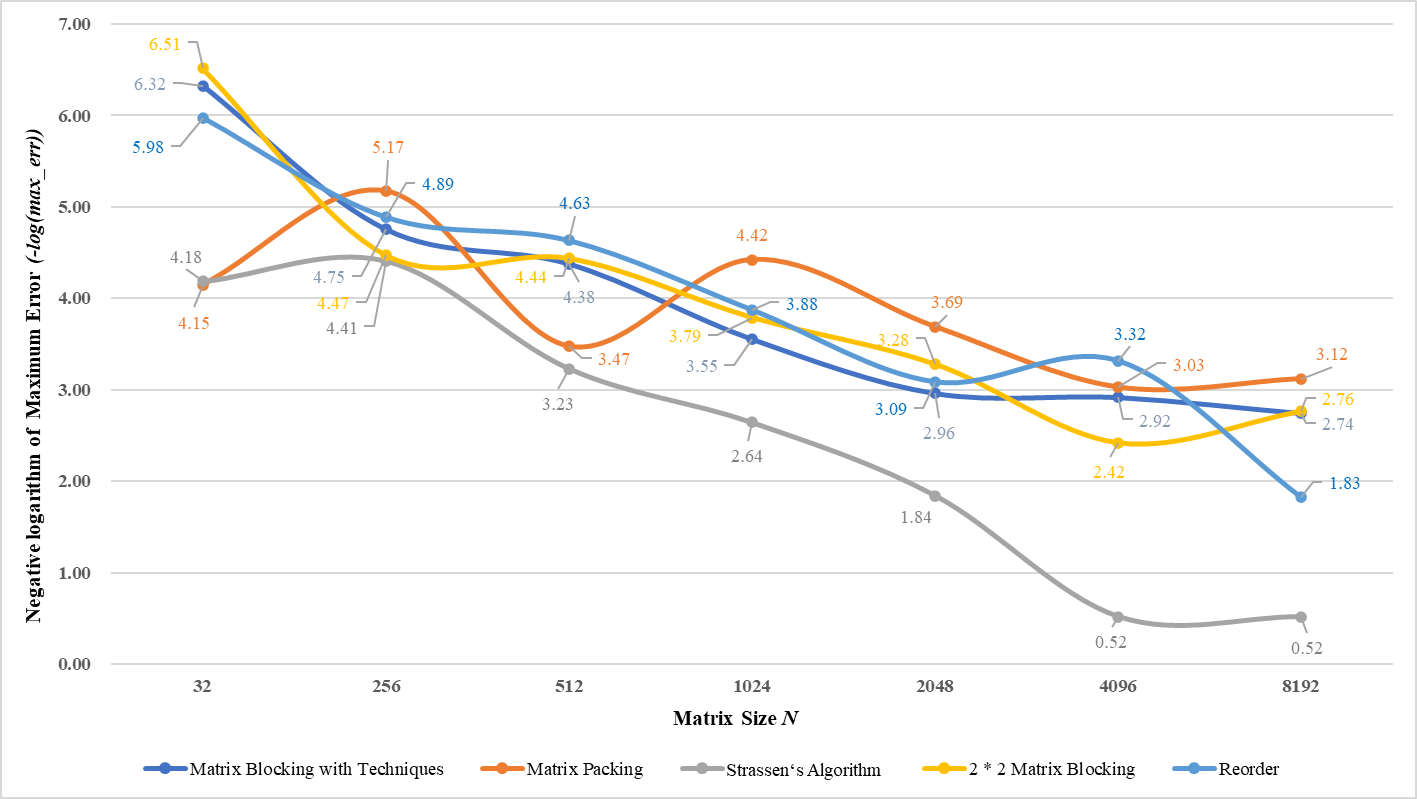
\includegraphics[width=0.5\textwidth]{fig10.png}}
		\caption{Error for Each Method}
		\label{fig::error}
	\end{figure}
	
	All aforementioned optimizations were successfully executed and ensured a certain level of accuracy compared to results obtained using the OpenBLAS library for a certain data scale. Of the aforementioned optimization methods, the Strassen's algorithm showed inadequate precision, as previously analyzed. The accuracy of the algorithms slightly declines as the data size increases, due to the precision limitations of float data types. However, experimentation has proven that this error remains within an acceptable range.
	
	\subsection{Different Platform}
	
	Based on the experimental results, we developed a matrix multiplication library that supports cross-platform execution on both x86 and ARM platforms. The former uses the SIMD instruction set for optimization, while the latter uses the NEON instruction set. Both platforms are optimized using OpenMP for parallelization. We conducted experiments on three devices and two platforms, and the results are presented in Figure.~\ref{fig::platform}.
	
	\begin{figure}[htbp]
		\centerline{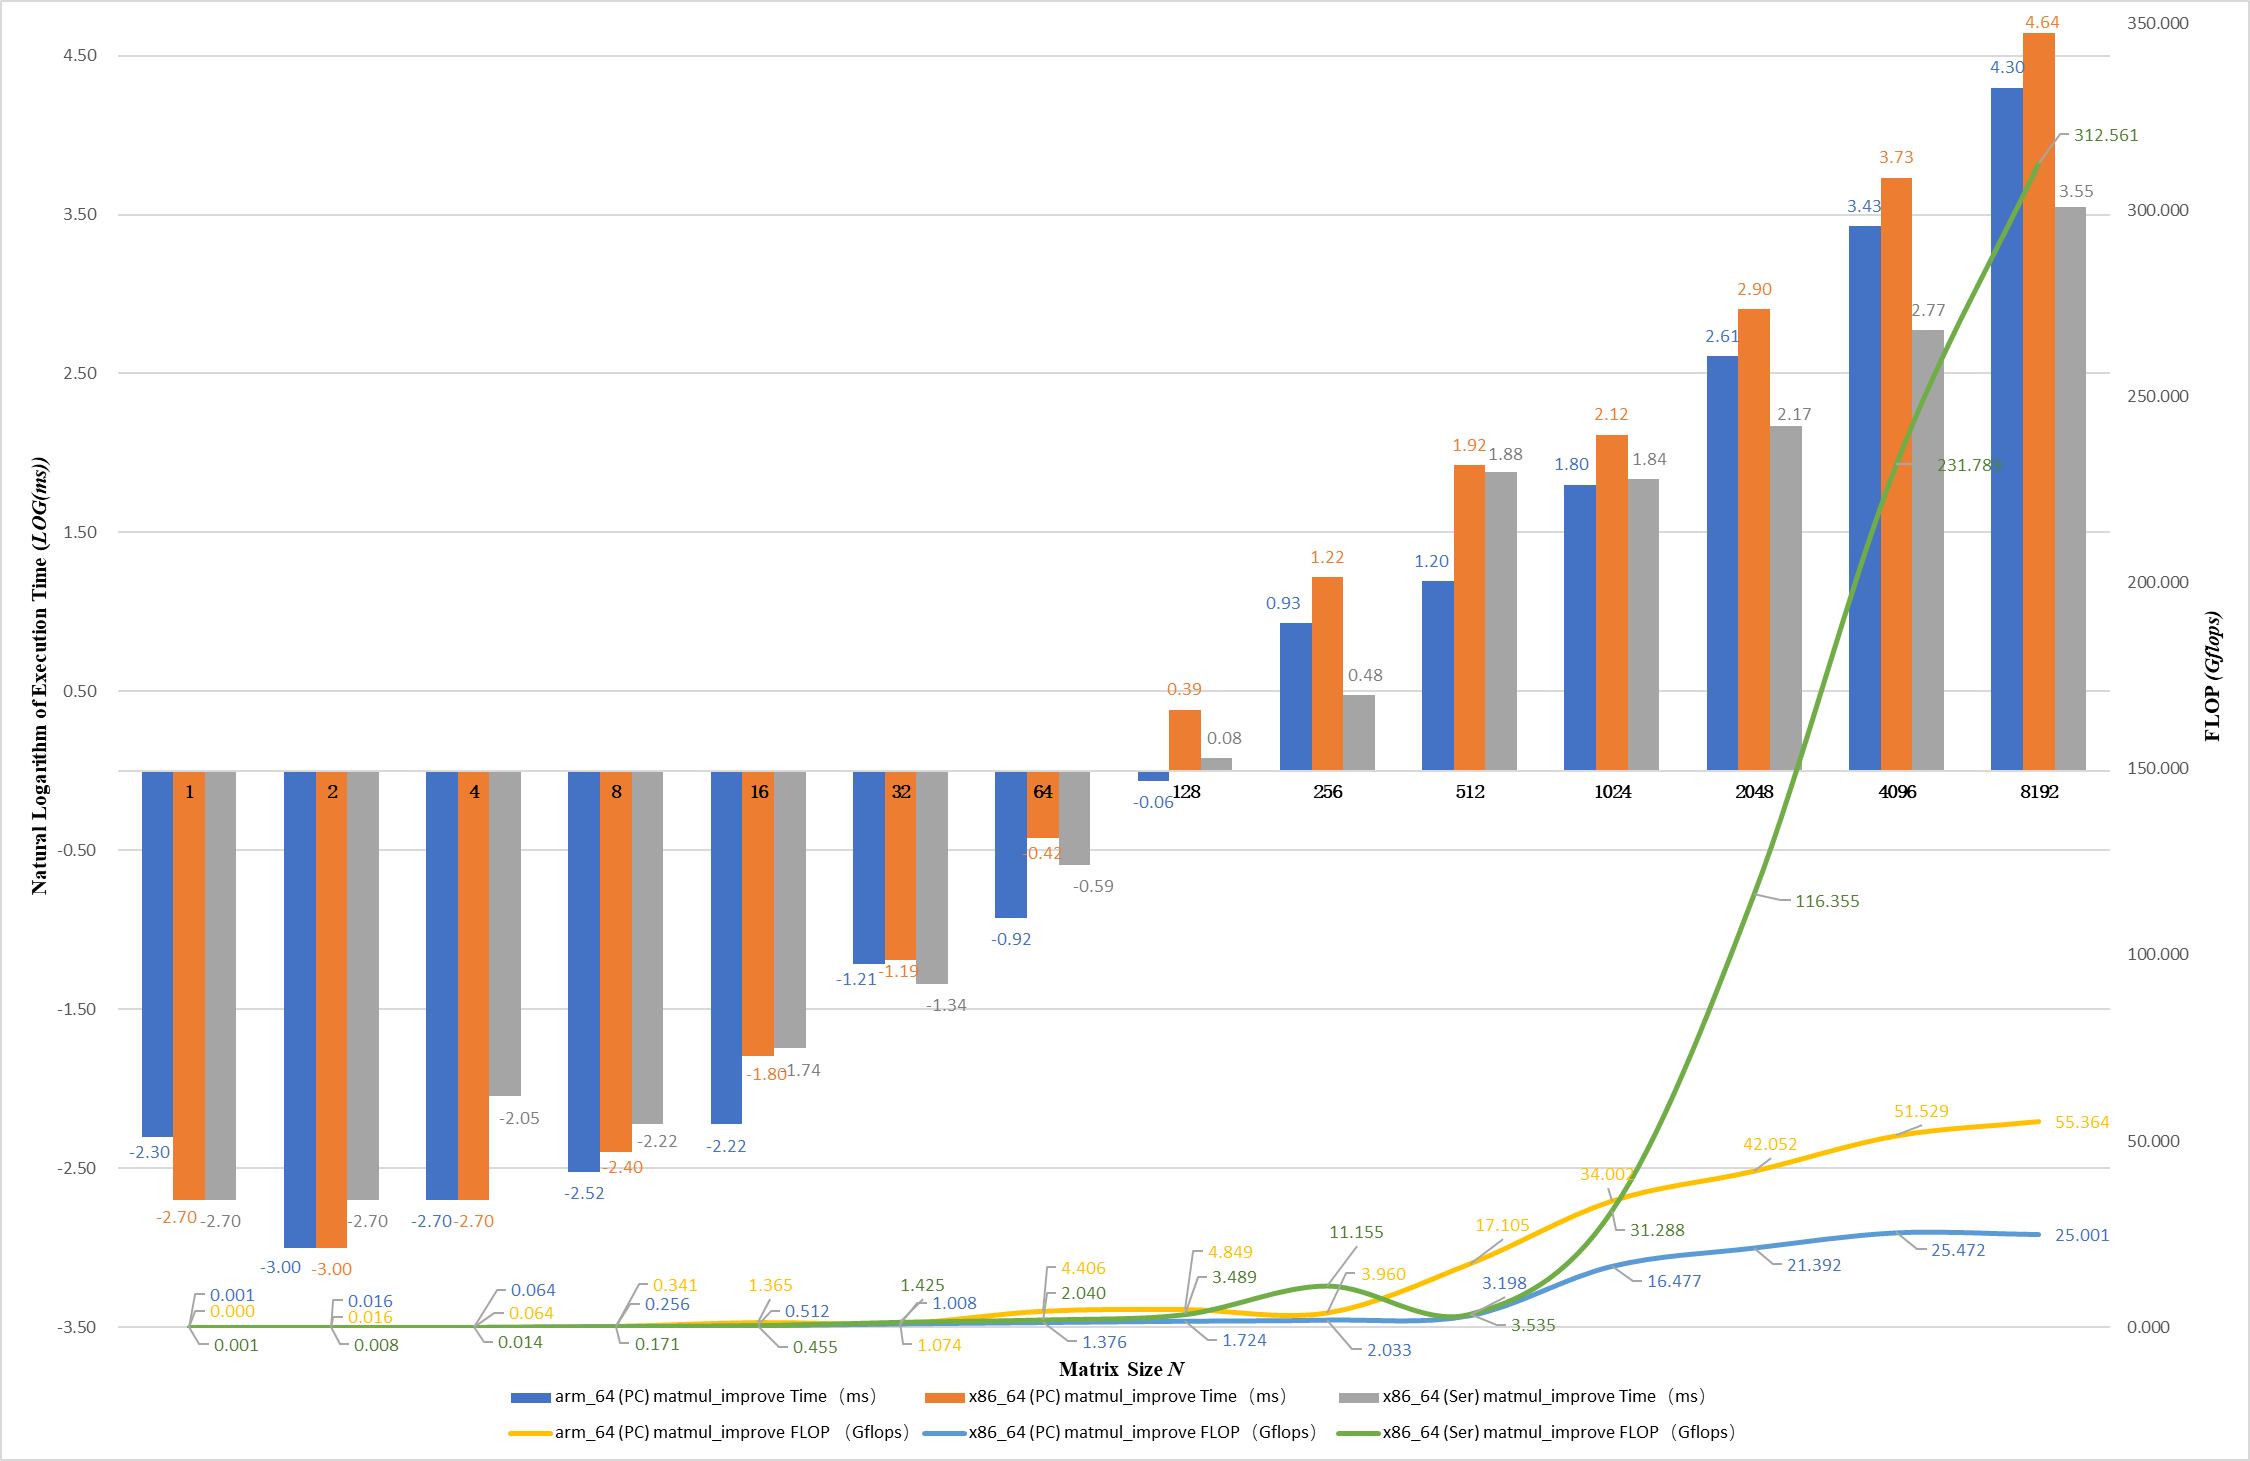
\includegraphics[width=0.5\textwidth]{fig11.png}}
		\caption{Efficiency Comparison Across Different Platforms}
		\label{fig::platform}
	\end{figure}

	The library was used to perform matrix calculations. For smaller matrix data sizes, matrix multiplication on ARM platforms proved to be more efficient than on x86 platforms, especially those with more cores, where efficiency was lower. For larger matrix data sizes, the efficiency markedly improved with more CPU cores, thanks to the use of multi-threading. Even with the same number of cores, ARM platforms demonstrated slightly higher efficiency than x86 platforms.
	
	Optimization for matrix multiplication was carried out using this library on different testing platforms, resulting in major improvements. However, the bottleneck effect was observed on x86 and ARM platforms with fewer cores, leading to stable floating-point frame rates.
	\section{Conclusion}
	
	In this work, we discovered that the naive matrix multiplication method does not fully utilize modern computer tiered architecture, resulting in significant data IO overhead and low efficiency. However, through appropriate data structure organization, parallelization, and instruction set optimization, the efficiency of naive matrix multiplication improved by over 2000 times. Other divide-and-conquer algorithms with lower time complexity were not suitable for practical matrix multiplication due to specific circumstances. Based on the matrix computing library proposed in this study, we can perform efficient cross-platform matrix calculations on both x86 and ARM platforms, which has significant potential.
	
	\begin{thebibliography}{00}
		\bibitem{b1} Cormen, Thomas H.; Leiserson, Charles E.; Rivest, Ronald L.; Stein, Clifford (2009) [1990]. Introduction to Algorithms (3rd ed.). MIT Press and McGraw-Hill. pp. 75–79. ISBN 0-262-03384-4.
		\bibitem{b2}  Skiena, Steven (2008). ``Sorting and Searching''. The Algorithm Design Manual. Springer. pp. 45–46, 401–3.
		\bibitem{b3} Amarasinghe, Saman; Leiserson, Charles (2010). "6.172 Performance Engineering of Software Systems, Lecture 8". MIT OpenCourseWare. Massachusetts Institute of Technology. Retrieved 27 January 2015.
		\bibitem{b5} Skiena, Steven S. (1998), "§8.2.3 Matrix multiplication", The Algorithm Design Manual, Berlin, New York: Springer-Verlag, ISBN 978-0-387-94860-7.
	\end{thebibliography}
\end{document}
